\newpage
\section*{Soluzione}

Lo scopo di questa esercitazione \`e fornire un esempio di
programmazione in cui vengono utilizzati i costrutti base del
linguaggio. Si riporta di seguito il listato del programma.
\lstset{basicstyle=\scriptsize\sf}
\lstinputlisting{./es/fin.cpp}
\lstset{basicstyle=\sf}

Oltre ai costrutti base comuni ai linguaggi di programmazione di alto
livello, il C++ offre una collezione di librerie standard che
implementano funzioni, classi, costanti ed oggetti di uso
frequente. Nel caso in esame sono state utilizzate le librerie
seguenti: \emph{iostream}, che implementa le classi per l'I/O sui
canali standard in ingresso ed uscita (\cpp{std::cin} e
\cpp{std::cout}); \emph{fstream}, che implementa le classi per
l'I/O su \emph{file}; \emph{cmath.h}, in cui sono definite le funzioni
matematiche di uso comune; \emph{vector}, che contiene
l'implementazione di un \cpp{template} \cpp{vector} per la
gestione degli \emph{array}. Si noti che la direttiva \cpp{using
namespace} \cpp{std} consente di accedere ai nomi del \cpp{namespace}
\cpp{std} omettendo la risoluzione esplicita, ovvero di scrivere
semplicemente \cpp{cout} in luogo di \cpp{std::cout}.

Le variabili globali sono state definite all'esterno del \emph{main
program}, in modo da essere visibili ovunque all'interno del
\emph{file}. L'attributo \cpp{const} indica al compilatore che la
variabile non pu\`o trovarsi al primo membro di un'assegnazione. Se
introducessimo l'istruzione: 
\lstset{basicstyle=\scriptsize\sf}
\begin{lstlisting}
const int MMAX = 501;
...
int main(){     
    MMAX = 30;
    ...
}
\end{lstlisting}
\lstset{basicstyle=\sf}
e tentassimo di compilare otterremmo il seguente messaggio d'errore:
\begin{verbatim}
fin.cpp: In function `int main()':
fin.cpp:44: error: assignment of read-only variable `MMAX'
\end{verbatim}
Lo stile dei commenti \`e conforme alla sintassi di Doxygen, un
\emph{software} per la generazione automatica della documentazione, di
cui si discuter\`a in un'esercitazione successiva.

All'inizio del programma viene richiesto all'utente di inserire il
numero $M$ di elementi della discretizzazione. \`E stato inserito un
semplice meccanismo di controllo che ripete la richiesta qualora il
numero di elementi sia inferiore a $1$ o superiore a $MMAX$. Tale
controllo \`e implementato mediante un ciclo con controllo in coda
\cpp{do ... while}.

L'elemento finito corrispondente alla soluzione approssimata viene
definito come un vettore di \cpp{double} mediante l'istruzione:
\lstset{basicstyle=\scriptsize\sf}
\begin{lstlisting}
vector<double> uh(M + 1);
\end{lstlisting}
\lstset{basicstyle=\sf}
che alloca lo spazio per $M+1$ elementi. La ragione per cui il tipo
degli elementi memorizzati nel vettore \`e dichiarato tra parentesi
angolari diverr\`a chiara quando verr\`a introdotto il concetto di
\cpp{template}. Per inizializzare il vettore si \`e utilizzato un
ciclo \cpp{for} in cui si accede agli elementi mediante
l'\cpp{operator[]} (\emph{accesso per indice}).

La scrittura su \emph{file} dei risultati sfrutta la class
\emph{ostream} e l'operatore di scorrimento \cpp{<<}. L'istruzione
\lstset{basicstyle=\scriptsize\sf}
\begin{lstlisting}
f.close();
\end{lstlisting}
\lstset{basicstyle=\sf}
chiude il canale di accesso al \emph{file}. In
\figref{fig:fin:results} la soluzione approssimata ottenuta mediante
il codice proposto discretizzando con $M=20$ elementi \`e confrontata
con la soluzione esatta.
%
\begin{figure}
\subfigure[Profilo di temperatura.]{
\psfrag{T}{$T$ ($\uK$)}
\psfrag{x}{$x$}
\psfrag{uh}{$u_h$}
\psfrag{u}{$\theta$}
\includegraphics[height=0.45\textwidth,angle=-90]{./figures/eps/fin.profile.eps}
}
\subfigure[Convergenza.]{
\psfrag{linf}{$\norm{ e }_{\hilbertL{\infty}{\Omega}}$}
\includegraphics[height=0.45\textwidth,angle=-90]{./figures/eps/fin.convergence.eps}
}
\caption{Soluzione approssimata ed esatta del problema definito dai
dati in \tabref{tab:parameters} e risultati sperimentali di convergenza.}
\label{fig:fin:results}
\end{figure}
